\section{Data Validity Validation}

This section evaluates whether the converted hospital-side records contain learnable information for image-conditioned robot motion prediction. The purpose is not to report a complete policy deployment result, but to verify that the synchronized ultrasound images and converted flange-motion labels can support supervised training of an imitation-learning model.

We used a diffusion-policy-style action-chunk predictor conditioned on ultrasound images. Each sample uses an ultrasound frame as the visual observation and predicts a future action chunk of flange pose deltas. The image encoder is a ResNet18 backbone, which maps the ultrasound frame into a visual conditioning vector. During training, Gaussian noise is added to the future pose-delta chunk according to a linear diffusion schedule, and an MLP denoiser predicts the injected noise from the noisy action chunk, the diffusion timestep embedding, and the ResNet18 image condition. In the current implementation, the action horizon is 20 and each action step is represented by a 7-dimensional flange pose delta.

Figure~\ref{fig:data_validity_diffusion_training} shows the training and validation mean-squared-error (MSE) noise-prediction losses. Both curves decrease rapidly during the early epochs and then converge more gradually, indicating that the model can extract a learnable relationship between ultrasound observations and future robot-frame motion labels. The best validation loss reaches 0.0664, and the final epoch reports a training loss of 0.0823 and a validation loss of 0.0803. The close train-validation behavior suggests that the converted dataset is not merely memorized by the model and provides usable supervision for downstream imitation learning. These results support the validity of the proposed data-conversion pipeline and motivate further evaluation with rollout-level and task-level metrics.

\begin{figure}[!htbp]
    \centering
    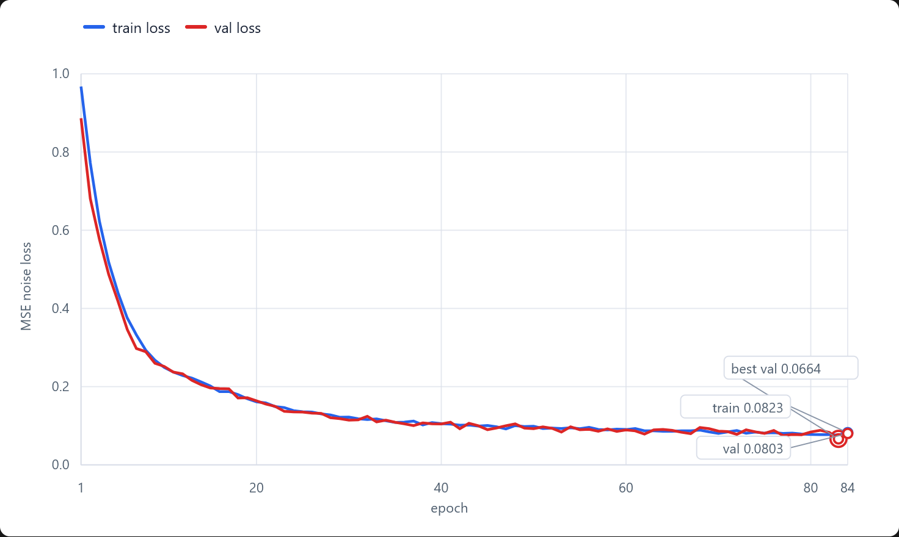
\includegraphics[width=\columnwidth]{figures/data_validity_diffusion_training.png}
    \caption{Data validity validation using a ResNet18-conditioned diffusion policy. The model is trained to predict diffusion noise for future flange pose-delta chunks from ultrasound image conditions. Training and validation MSE losses decrease consistently, with the best validation loss reaching 0.0664 and the final epoch reporting 0.0823 training loss and 0.0803 validation loss.}
    \label{fig:data_validity_diffusion_training}
\end{figure}
